\section{Conclusion} \label{Conclusion}

This paper has assessed the consumption-based asset pricing model's ability to rationalise observed financial returns when accounting for disaster risk. Comprehensively analyzing a newly available dataset by \citet{Jorda2017} which covers almost 150 years of financial and macroeconomic history of 16 developed countries and deploying a richer preference specification of the EZW-class that disentangles the preference parameters with respect to marginal utility in the intratemporal (risk aversion) and intertemporal (IES) space showed to yield implied preference parameters which accord with theoretical insights and attenuate the equity risk premium puzzle by a considerable proportion. Having itentified heterogeneity with respect to risk-sharing capacity and risk preference across countries lays path to a departure towards policy-related studies addressing the roles of fiscal capacity, market regulation and globalisation, to name just a few.


%With ongoing globalisation and financial integration countries should converge towards full consumption insurance. 
Conventional measures of aggregate consumption show still too high idiosyncratic consumption volatility (conditional on output) and too low international consumption correlations which ``have remained approximately constant after 1980 and and thoughout the 1990s'' \cite{Artis2008} which is known as the \textit{risk-sharing puzzle}.
\citet{Cochrane1991} compares the basic idea of consumption insurance as the cross-sectional counterpart of the permanent income hypothesis, i.e. aggregate consumption of any individual country does not vary in response to idiosyncratic income shocks. A competitive equilibrium requires markets to be complete and/or institutional arrangements implementing optimal allocations \cite{Canova1996}. In the context of disaster risk those arrangements (e.g. charities, disaster relief programs, international lending agreements or direct foreign aid) do exist in reality but were put in place successively in response to the most severe disasters in modern history. Systemic crises pose significant distortions to optimal consumption allocations across countries with strong persistence. \citet{Canova1996} empirically argue that consumption correlations are not perfect (meaning that marginal utility of consumption is not equalized across countries) and that countries with closer economic ties (E.E.C. back then) ``may also have more efficient risk sharing mechanisms.''\footnote{They also provide estimates of CRRA coefficients for the representative agent in each country (relative to the U.S.) for eight developed countries which deviate substantially from the ones reported in this paper.}, contrasting the theoretical implications of international business cycle (IBC) models such as in \citet{Backus1992}. \citet{Epstein2016} empirically test consumption, asset and labor income tax differentials within this class of models and argue that accounting for taxation does explain time-varying degree of risk sharing (and hence time-varying degree of risk-aversion).

After controlling for disaster risk the implied coefficients of relative risk aversion as in the baseline calibration may be subject to country-specific factors (or histories of policies) shaping the economic environment. \citet{Cui2016} models market liquidity explicitly as an endogeneous process of competetive search and match that gives rise to optimal monetary-fiscal interaction. Public liquidity in form of government bonds may be also subject to liquidity risk, that is the degree of easiness of trading an asset and the price's sensitivity to the trades. Weak fiscal capacity therefore does not only increase the probability of default but also government bonds are less desirable, agents cannot fully self-insure through muted precautionary savings effects which induces them to require a higher premium. Fiscal capacity can be captured by the tax revenue to GDP ratio\footnote{Also taken from JST dataset} which accurately describes economic policy since both move one-by-one with the business cycle. 

\begin{figure}[H]
	\centering
  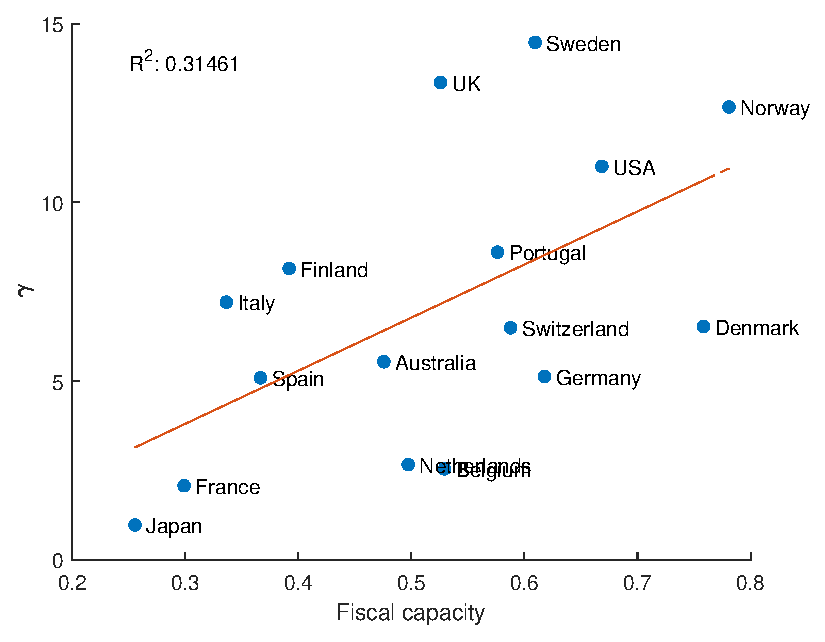
\includegraphics[width=0.7\textwidth]{Matlab Graphics/Fiscal_capacity}
	\caption{Standardized coefficients of variation, within-country tax revenue/GDP}
	\label{fig:fiscal_capacity}
\end{figure}
Figure \ref{fig:fiscal_capacity} above indicates that after controlling for disaster risk there is some variation stemming from fiscal capacity measured as the standardized coefficients of variation of within-country tax revenue/GDP. The higher the coefficient, the more the economic environment fluctuates and imposes distortions to financial markets, leading to liquidity premiums which leads to higher risk aversion. Further research could study different taxation types in the cross-section.

As \citet{Barro2006} suggests the analysis of real rates of return might include housing as component of the wealth portfolio as well. Given that such data is available \cite{Jorda2017} the implementation should be straight-forward.

\citet{Barro2006} and \citet{Nakamura2013} point at incorporating time-varying disaster moments which has been followed by \citet{Tsai2015}. The finding of \citet{Nakamura2013} on the role of the IES (especially at the onset of disasters) points at time-varying properties of the IES itself. Apart from dynamic aspects of disasters they also point out the distinction between actual and perceived disaster risks due to learning in order to alleviate the uncertainty regarding disaster parameters.